\documentclass[11pt]{amsart}

\usepackage{graphicx}
\usepackage{amsmath,amssymb,url}
\usepackage{bbm}
\usepackage{geometry}              
\usepackage{graphicx}
\usepackage{amssymb}
\usepackage{epstopdf}
\usepackage{tikz}
\usepackage{float}
\usepackage{amsthm}
\usepackage{graphicx}
\usetikzlibrary{matrix}
\usetikzlibrary{arrows}
\usepackage{algorithm}
\usepackage{algorithmic}
\usepackage{cancel}
\usepackage{amsmath}
\usetikzlibrary{calc} 
\usepackage{float}
\usepackage{fancyvrb}
\usepackage{tabularx}
\usepackage{subfig}
\usepackage{array}
\usepackage{color}
\usepackage[T1]{fontenc} 
\usepackage{fancyhdr}
\usepackage{enumitem}
\usepackage{mleftright}
\usepackage{comment}
\usepackage{caption}
\usepackage{wrapfig}
\usepackage{tikz-cd}
\usepackage{bbm}
\DeclareMathOperator\arctanh{arctanh}
\usepackage{pstricks}
\setcounter{MaxMatrixCols}{30}
\usetikzlibrary{decorations.pathreplacing,decorations.markings}
\usepackage{wasysym}

\usepackage{pst-solides3d}
\newcommand{\ndiv}{\centernot \mid}
\newcommand{\N}{\mathbb{N}}
\newcommand{\R}{\mathbb{R}}
\newcommand{\Z}{\mathbb{Z}}
\newcommand{\Q}{\mathbb{Q}}
\newcommand{\C}{\mathbb{C}}
\newcommand{\norm}{\mathcal{N}}
\newcommand{\E}{\mathcal{E}}
\newcommand{\F}{\mathcal{F}}

\newcommand{\bigslant}[2]{{\raisebox{.2em}{$#1$}\left/\raisebox{-.2em}{$#2$}\right.}}
\newcommand{\overbar}[1]{\mkern 1.5mu\overline{\mkern-1.5mu#1\mkern-1.5mu}\mkern 1.5mu}
\usepackage{amsthm}
%\theoremstyle{remark}
\newtheorem{theorem}{Theorem}[section]
\newtheorem{lemma}[theorem]{Lemma}
\theoremstyle{definition}
\newtheorem{defn}[theorem]{Definition}
\newtheorem{ex}[theorem]{Example}
\usetikzlibrary{positioning}
\usepackage{hyperref}
\usetikzlibrary{shapes.geometric}
\usetikzlibrary{shapes.misc}
%\usetikzlibrary{arrows.meta}
\setlist[enumerate]{leftmargin=.15in}
\newcolumntype{L}{>$l<$}
\tikzset{
  % style to apply some styles to each segment of a path
  on each segment/.style={
    decorate,
    decoration={
      show path construction,
      moveto code={},
      lineto code={
        \path [#1]
        (\tikzinputsegmentfirst) -- (\tikzinputsegmentlast);
      },
      curveto code={
        \path [#1] (\tikzinputsegmentfirst)
        .. controls
        (\tikzinputsegmentsupporta) and (\tikzinputsegmentsupportb)
        ..
        (\tikzinputsegmentlast);
      },
      closepath code={
        \path [#1]
        (\tikzinputsegmentfirst) -- (\tikzinputsegmentlast);
      },
    },
  },
  % style to add an arrow in the middle of a path
  mid arrow/.style={postaction={decorate,decoration={
        markings,
        mark=at position .5 with {\arrow[#1]{stealth}}
      }}},
}
\tikzset{->-/.style={decoration={
  markings,
  mark=at position .5 with {\arrow{>}}},postaction={decorate}}}
\tikzset{->>-/.style={decoration={
  markings,
  mark=at position #1 with {\arrow{>}}},postaction={decorate, double}}}

\newfont{\bssdoz}{cmssbx10 scaled 1200}
\newfont{\bssten}{cmssbx10}
\newcommand{\B}{\mathcal{B}}
\newcommand{\pspace}{(\Omega, \mathcal{F},\mathbb{P})}
\newcommand{\p}{\mathbb{P}}
\newcommand{\diam}{\text{diam}}

%\oddsidemargin  0in \evensidemargin 0in \topmargin -0.5in
%\headheight 0.25in \headsep 0.25in
%\textwidth   6.5in \textheight 9in %\marginparsep 0pt \marginparwidth 0pt
%\parskip 1.5ex  \parindent 0ex \footskip 20pt


\begin{document}

\title{CME 211 HW4 Write Up}
\author{Laura Lyman}

\maketitle
\vspace{-20pt}
\tableofcontents
\section{Code Description} The class \texttt{Truss} returns a data table of the net force acting on each beam. That is, this class creates a system of linear equations by balancing the $x$ and $y$ forces acting on each joint, where the forces provided
by the beams are variables. Then the class solves this system of equations to determine each beam force and outputs the results in a data table. If the system cannot be solved (i.e. there is a singular matrix or non-square matrix) the class returns an error with an explanation.

Also, if the user inputs an (optional) file name, the code creates a figure of the truss system and saves it as that name. (If no directory is included in part of the file name, the default is to save the plot as the given name in the current directory.) Each figure is a picture of the corresponding joints/beam system, regardless of whether the associated matrix equation has a solution.

Specifically, here is a description of some of the methods in the Truss class.
\\ \\
%e details like the type of sparse matrix used and the input and output arguments for each method.
\centerline{$\begin{array}{||l||} \hline \hline
\text{Method: } \texttt{\_init\_(self, joints\_file,beams\_file, plot\_file)} \\
\text{Returned Variables: None} \\
\textbf{Description: }  \text{Initializes the class and its methods. Gives the Truss class attributes \texttt{joints\_file} } \\
\text{and \texttt{beams\_file} from the user-inputted data files. Also gives the Truss class a \texttt{plot\_file} attribute, } \\
      \text{which is where the plot should be
        saved/what to name the plot if the user specifies a file } \\
        \text{path; otherwise \texttt{plot\_file} is an empty string. Then the class
        methods are initialized.} \\ \hline \hline
%\text{if the user entered no plot name, \texttt{plot\_file} is an empty string.}   \\ \hline \hline
\text{Class Method: } \texttt{get\_beam\_data(self,beams\_file) } \\
\textbf{Description: }  \text{Creates the \texttt{beam\_joints} attribute, which is a dictionary in which the keys are beams} \\
\text{and the values are the joint indices of the two joints per each beam. The method reads through the}  \\
\texttt{beams\_file} \text{ line by line, storing all the information from this file in the \texttt{beam\_joints} dictionary.} \\ \hline \hline
\text{Class Method: } \texttt{get\_joints\_data(self,joints\_file)}\\
\textbf{Description: }  \text{Reads and retrieves information from the joints data file. This method adds three } \\
\text{class attributes that are all dictionaries and populates them with data: } \texttt{joints\_with\_attached\_beams}, \\\texttt{joint\_position}, \text{ and } \texttt{joint\_forces}. \text{ Each of these dictionaries have the joints  (i.e. joint indices) as} \\
\text{keys, which are } \text{unique identifies. Then: } \\
\bullet \ \texttt{joints\_with\_attached\_beams} \text{ has values that are the beam indices of the beams } \\
\text{attached to each joint} \\
\bullet \ \texttt{joint\_position} \text{ has values that are the $(x,y)$ coordinates for each joint, and} \\
\bullet \texttt{joint\_forces} \text{ has values that are lists including: the $x$-forces on each joint, } \\
\text{ the $y$-forces
        on each joint, and a boolean for whether each joint
        is attached to a wall.} \\ \hline \hline
\text{Class Method: }  \texttt{get\_beam\_length(self)} \\
\textbf{Description: }  \text{Creates two dictionaries \texttt{beam\_lengths} and \texttt{beam\_trig}, whose keys are joint indices.} \\
\text{Uses trigonometry to compute the length of each beam (populating \texttt{beam\_lengths}). Computes the} \\
\text{sine and cosine of the angles of a beam (relative to the first joint) and puts these two values into a list;} \\
\text{then \texttt{beam\_trig} is populated with these lists of angle information. }  \\ \hline \hline
\text{Class Method: }  \texttt{check\_if\_square(self)} \\
\textbf{Description: }  \text{Checks if the matrix of data is square. Throws an error if
        the matrix is rectangular } \\
        \text{i.e. the number of
        equations ($m$) does not equal the number of
        variables ($n$). There are 2 equations } \\
        \text{per joint. There is one variable per beam. Also, there are two
        additional variables per attached } \\
        \text{joint representing
        the force of attachment in the $x$ and $y$ directions. So the total number of variables } \\
        \text{is \texttt{number\_of\_beams + 2*number\_attached\_joints}.} \\ \hline \hline
\end{array} $}
\\ \\
The beam equations are then balanced by \texttt{get\_beam\_eqn(self)}, stored into CSR arrays (\texttt{update\_CSR\_arrays}), and put into a CSC matrix using \texttt{scipy.sparese.csc\_matrix}. Then \texttt{check\_for\_singular\_matrix} checks if this CSC matrix is singular (to know whether a solution can be found) and outputs an error if needed. The \texttt{solve\_linear\_system} method solves for the forces on each beam using \texttt{scipy.sparse.linalg.spsolve}, and \texttt{PlotGeometry} handles the figures of each truss system. The code in \texttt{truss.py} contains detailed comments describing all of the other helper functions used. 

\section{Table Results (Beam/Force Tables)}
\begin{Verbatim}[fontsize=\small]
$ python3 main.py truss1/joints.dat truss1/beams.dat
 Beam       Force
-----------------
    1       0.000
    2      -1.000
    3       0.000
    4      -1.000
    5       0.000
    6       0.000
    7       0.000
    8      -1.414
$ python3 main.py truss2/joints.dat truss2/beams.dat
 Beam       Force
-----------------
    1   -2000.044
    2    1732.102
    3     866.032
    4   -2500.055
    5   -2020.741
    6    3175.520
$ python3 main.py truss3/joints.dat truss3/beams.dat
ERROR: Linear system is not square. Method of joints isn't suitable.
$ python3 main.py truss4/joints.dat truss4/beams.dat
ERROR: Matrix is singular, so linear system cannot be solved.
\end{Verbatim}
\section{Plotting Results}
The plots of the truss systems are below.
\begin{figure}[h]
\centerline{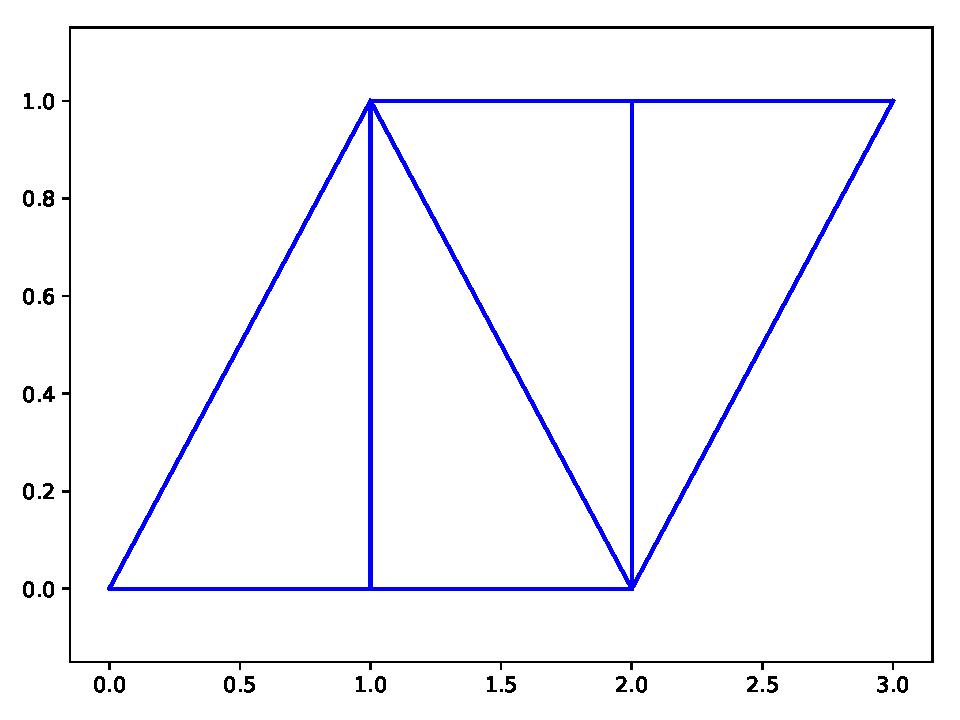
\includegraphics[scale=.4]{Figure1.pdf} 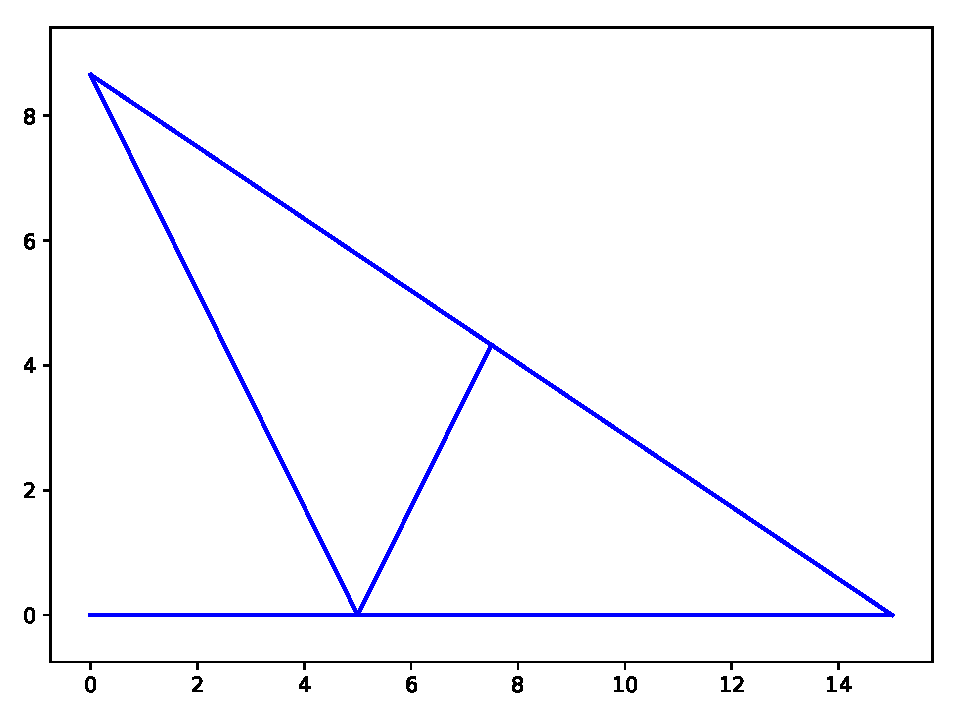
\includegraphics[scale=.4]{Figure2.pdf}}
\caption{Plots of truss system 1 (left) and truss system 2 (right).}
\end{figure}
\begin{figure}[h]
\centerline{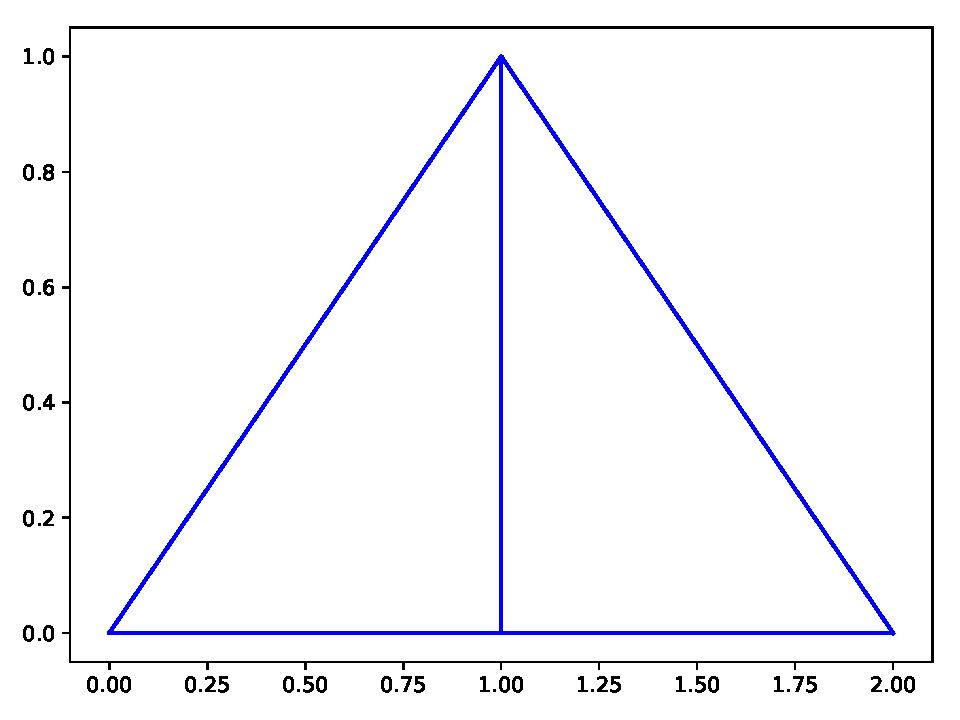
\includegraphics[scale=.4]{Figure3.pdf} 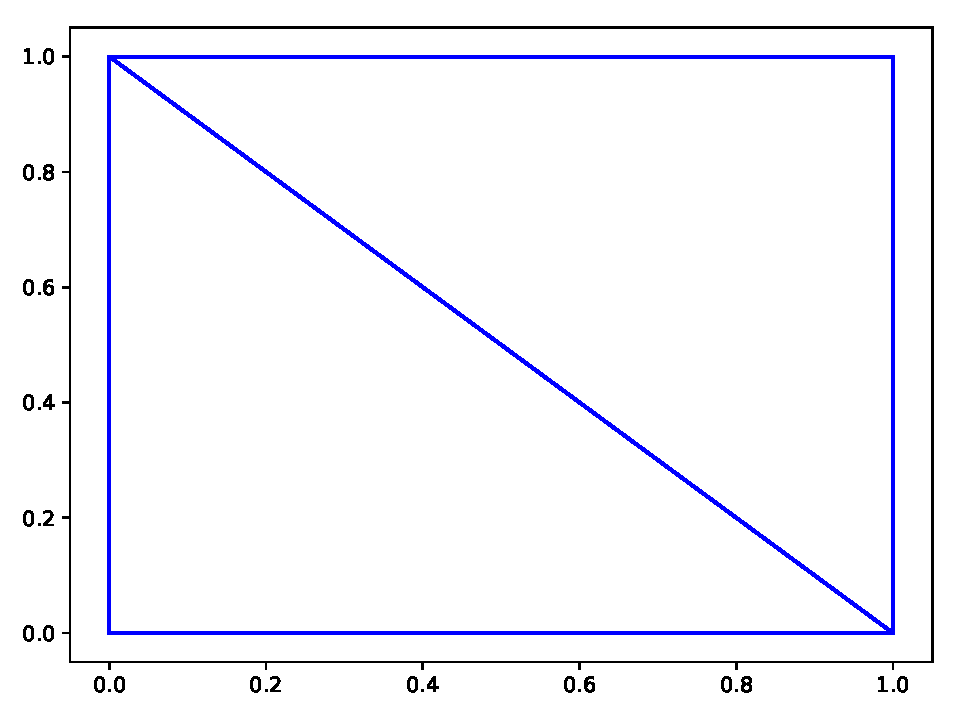
\includegraphics[scale=.4]{Figure4.pdf}}
\caption{Plots of truss system 3 (left) and truss system 4 (right).}
\end{figure}


\section{Error Handling}
Here we verify that an error is thrown if the inputted joints or beam file has formatting issues that will cause the file to not be found by \texttt{os.path} (i.e. ``correct" file names but excessive `/' characters).
\begin{Verbatim}[fontsize=\small]
$ python3 main.py /truss1/joints.dat truss1/beams.dat
ERROR: Make sure `/truss1/joints.dat' does not start or end with a `/' character.

$ python3 main.py truss1/joints.dat truss1/beams.dat/
ERROR: Make sure `truss1/beams.dat/' does not start or end with a `/' character.
\end{Verbatim}

Then we verify that an error is thrown if the inputted joints or beams file is located in a nonexistent directory.
\begin{Verbatim}[fontsize=\small]
$ python3 main.py truss5/joints.dat truss1/beams.dat
ERROR: File `truss5/joints.dat' not found.
\end{Verbatim}
The following checks how the code handles a reference to a nonexistent file in one of the valid directories.\begin{Verbatim}[fontsize=\small]
$ python3 main.py truss1/joints.dat truss1/filenothere
ERROR: File `truss1/filenothere' not found.
\end{Verbatim}
When the user specifies a valid directory without a file, the error is caught under the formatting issues umbrella.
\begin{Verbatim}[fontsize=\small]
$ python3 main.py truss1/joints.dat truss1/
ERROR: Make sure `truss1/' does not start or end with a `/' character.
\end{Verbatim}
We can check how the code handles these similar file issues when the user specifies a plot file name.
\begin{Verbatim}[fontsize=\small]
$ python3 main.py truss1/joints.dat truss1/beams.dat /myplotfile
ERROR: Make sure `/myplotfile' does not start or end with a `/' character.
$ python3 main.py truss1/joints.dat truss1/beams.dat truss10/myplotfile
ERROR: Directory `truss10' not found.
$ python3 main.py truss1/joints.dat truss1/beams.dat /truss5/fig
ERROR: Make sure `/truss5/fig' does not start or end with a `/' character.
\end{Verbatim}
Finally we need to verify that you can actually specify a plot file name and have the plot saved accordingly. If you have a certain directory in the plot file name (that is valid), we will check that the plot is actually saved there. If no directory is specified (i.e. the user just says ``fig1"), we will check that the plot is saved as ``fig1" in the current directory. Note that if no extension is provided by the user for the plot, the plot is saved as a `.png' by default. Finally, we should ensure that tables are still working/outputting correctly now that a plot file has been provided.
\begin{Verbatim}[fontsize=\small]
$ python3 main.py truss2/joints.dat truss2/beams.dat testfig2
 Beam       Force
-----------------
    1   -2000.044
    2    1732.102
    3     866.032
    4   -2500.055
    5   -2020.741
    6    3175.520
$ ls
Figure1.pdf        README.synctex.gz       testfig2.png
Figure2.pdf        README.tex              truss3
Figure3.pdf        README.toc              truss4
Figure4.pdf        cme211-hw4.pdf	
README.aux	 main.py		
README.log	 truss.py	
README.out	 truss1
README.pdf	 truss2

$ python3 main.py truss1/joints.dat truss1/beams.dat truss1/testfig.pdf
 Beam       Force
-----------------
    1       0.000
    2      -1.000
    3       0.000
    4      -1.000
    5       0.000
    6       0.000
    7       0.000
    8      -1.414
$ cd truss1
$ ls
beams.dat	joints.dat	testfig.pdf
$ cd ..
$ python3 main.py truss3/joints.dat truss3/beams.dat fig
ERROR: Linear system is not square. Method of joints isn't suitable.
$ python3 main.py truss4/joints.dat truss4/beams.dat fig
ERROR: Matrix is singular, so linear system cannot be solved.
\end{Verbatim}
Therefore, the program appears to work correctly and manage several types of errors.
\end{document}
